\section{Experimental results}
\label{section:results}
We have implemented the algorithms in C++ and conducted the experiments
on Linux PCs with Intel Core i7 processor with 4 cores, enabling 8 threads
with the hyper threading technology. We have used the Graph-cuts
optimization code written by Veksler, using the libraries provided by
Boykov and Kolmogorov~\cite{middle_bury,2,3,4_below}.
% [2] Fast Approximate Energy Minimization via Graph Cuts.
%         Y. Boykov, O. Veksler, and R. Zabih.
%         In IEEE Transactions on Pattern Analysis and Machine Intelligence
%         (PAMI), vol. 23, no. 11, pages 1222-1239, November 2001.  
%
%     [3] What Energy Functions can be Minimized via Graph Cuts?
%         V. Kolmogorov and R. Zabih. 
%         In IEEE Transactions on Pattern Analysis and Machine Intelligence
%         (PAMI), vol. 26, no. 2, pages 147-159, February 2004. 
%         An earlier version appeared in European Conference on Computer
%         Vision (ECCV), May 2002.
%
%     [4] An Experimental Comparison of Min-Cut/Max-Flow Algorithms for
%         Energy Minimization in Vision. 
%         Y. Boykov and Vladimir Kolmogorov.
%         In IEEE Transactions on Pattern Analysis and Machine Intelligence
%         (PAMI), vol. 26, no. 9, pages 1124-1137, September 2004. 
We have used the QPBO and TRW-S implementations by
Kolmogorov~\cite{msr_link?,trw_link}.



The figure illustrates the convergence rate of three competing methods
(alpha expansion, parallel alpha expansion, hierarchical fusion) against
our swarm fusion method (only binary fusion without proposal
generation \chen{We generate proposals on the fly for optical flow and layered depth map. So the time actually includes proposal generation stage which can be ignored. I think we can just delete this sentence.}).

%\hang{figure file missing}
\begin{figure}[tb]
  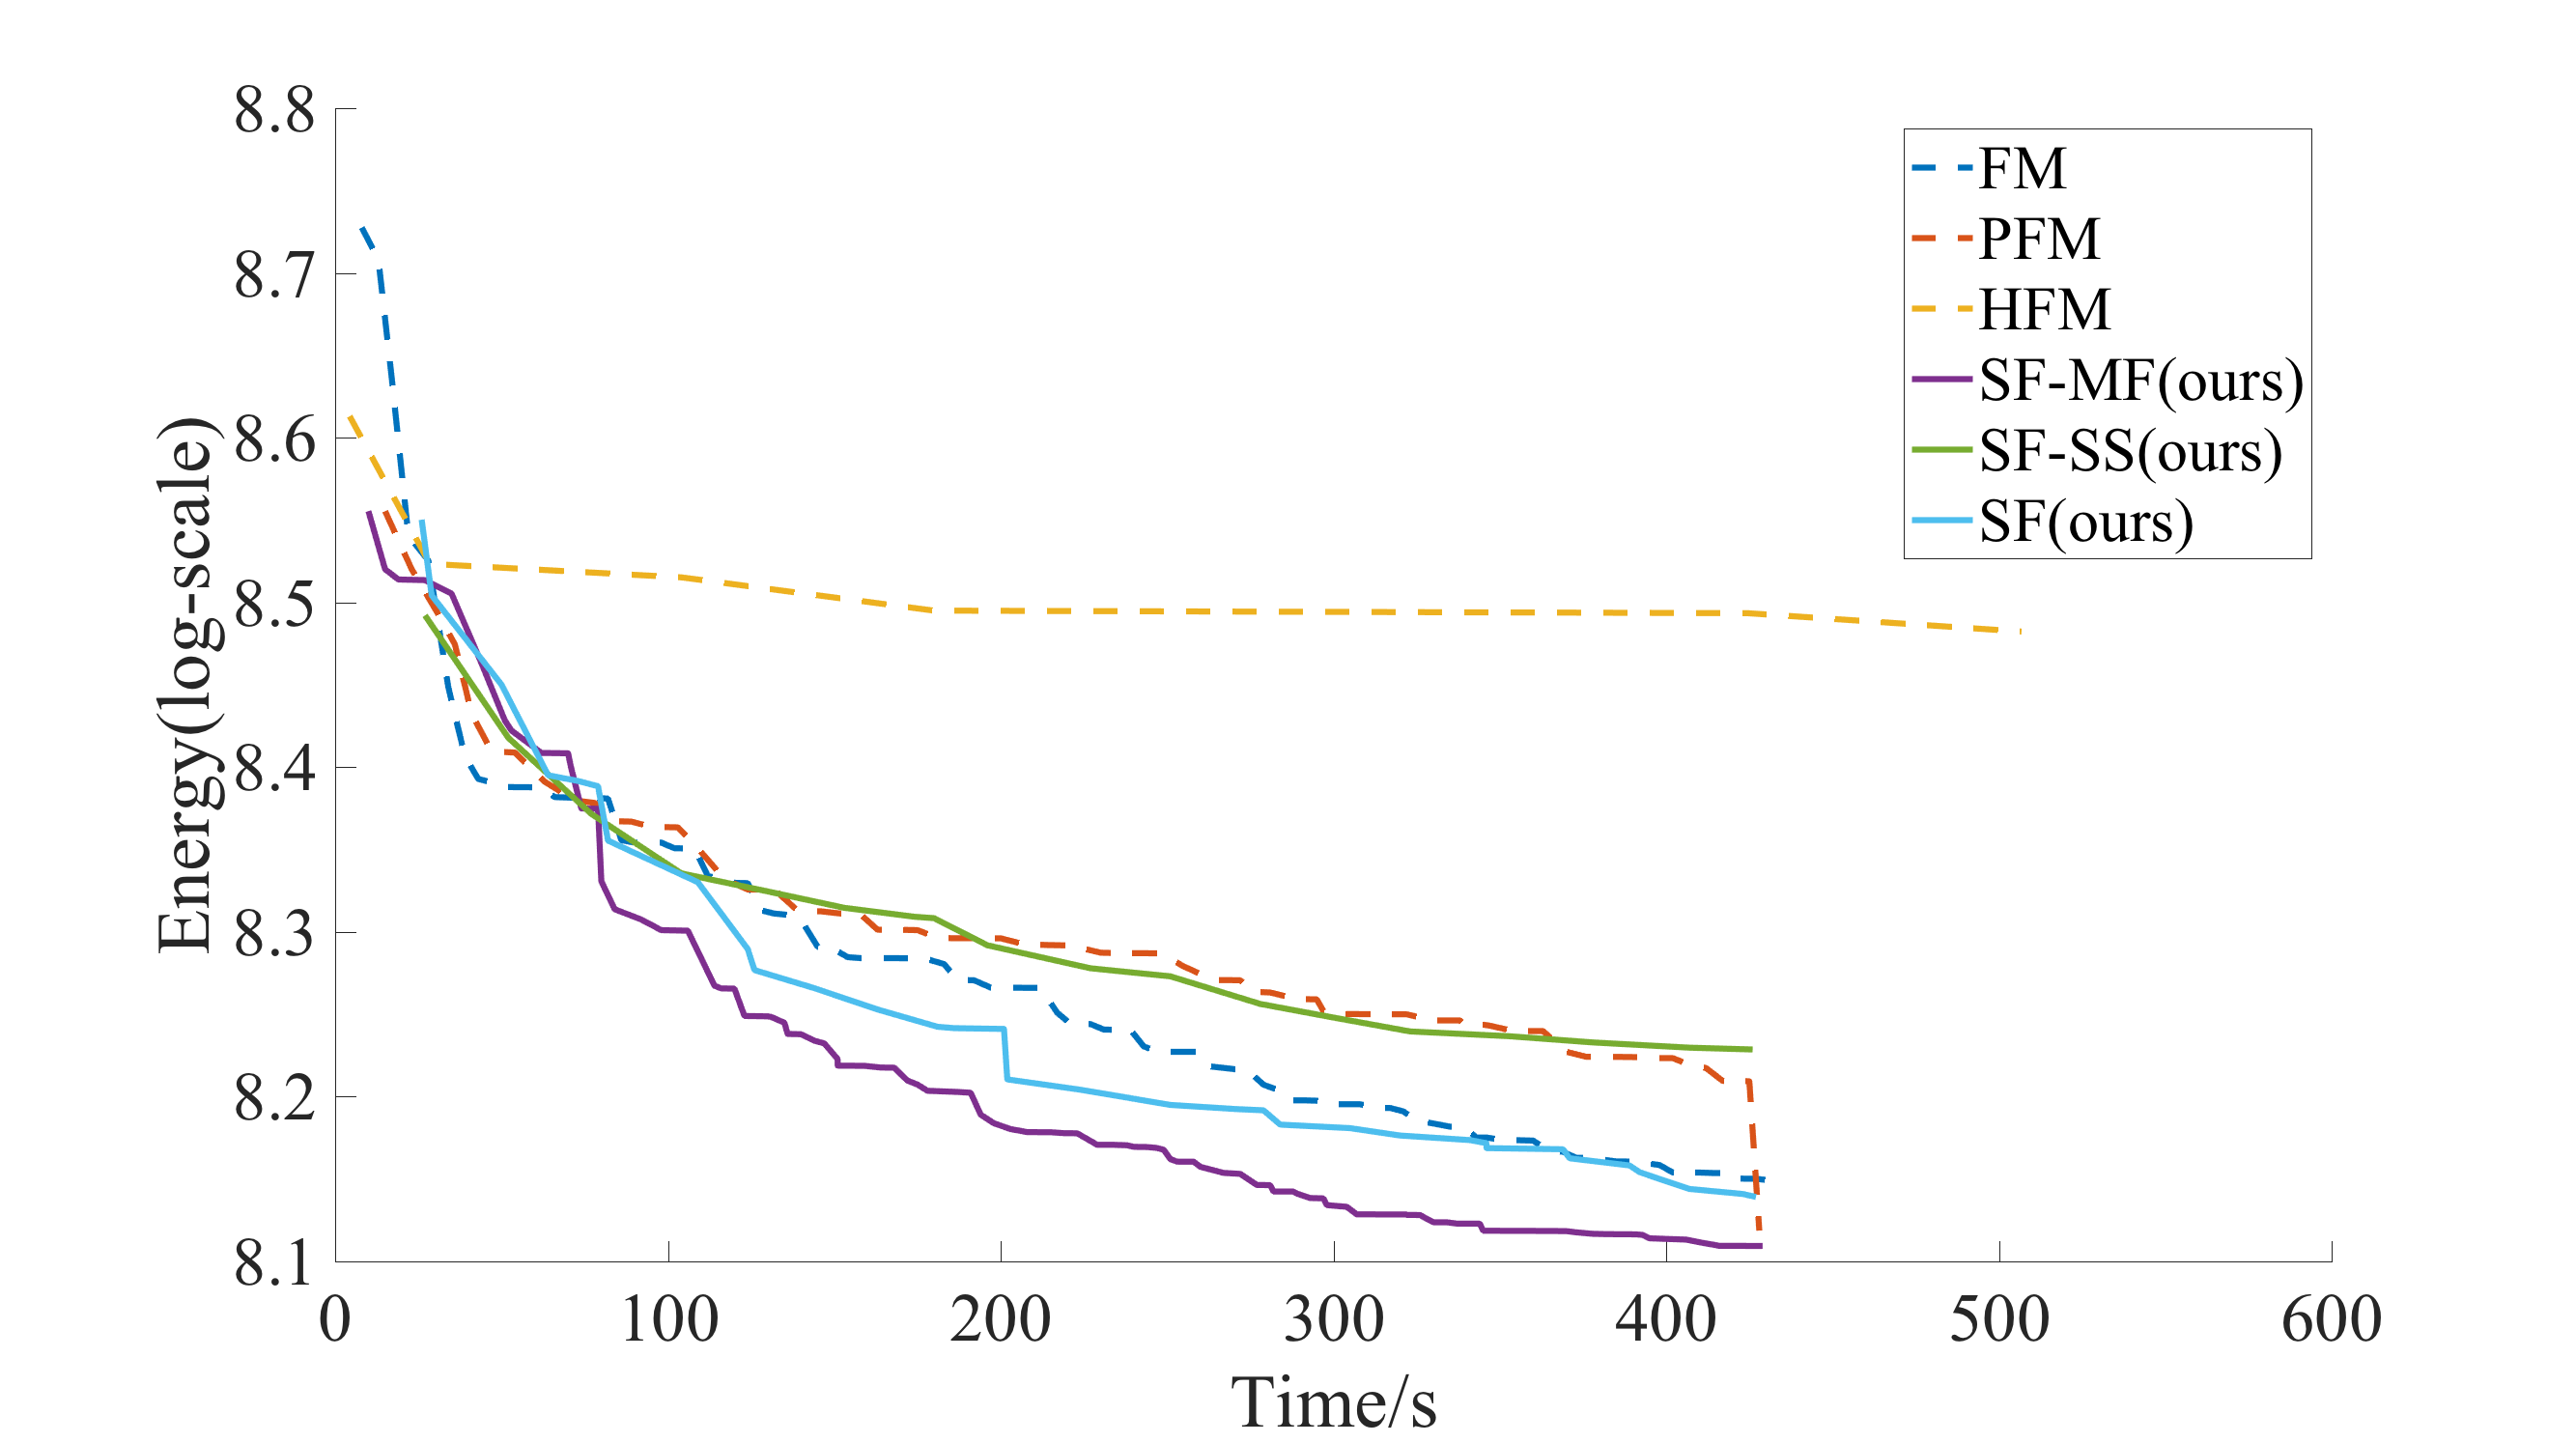
\includegraphics[width=\columnwidth]{figure/optical_flow_convergence.png}
  \caption{}\label{fig:optical_flow_convergence}
\end{figure}
\begin{figure}[tb]
 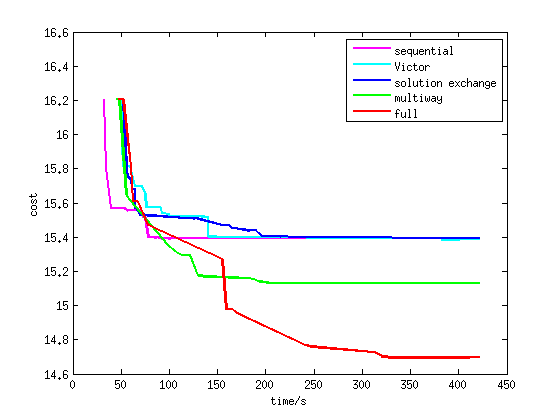
\includegraphics[width=\columnwidth]{figure/layered_depthmap_convergence.png}
 \caption{}\label{fig:layered_depthmap_convergence}
\end{figure}
\begin{figure}[tb]
  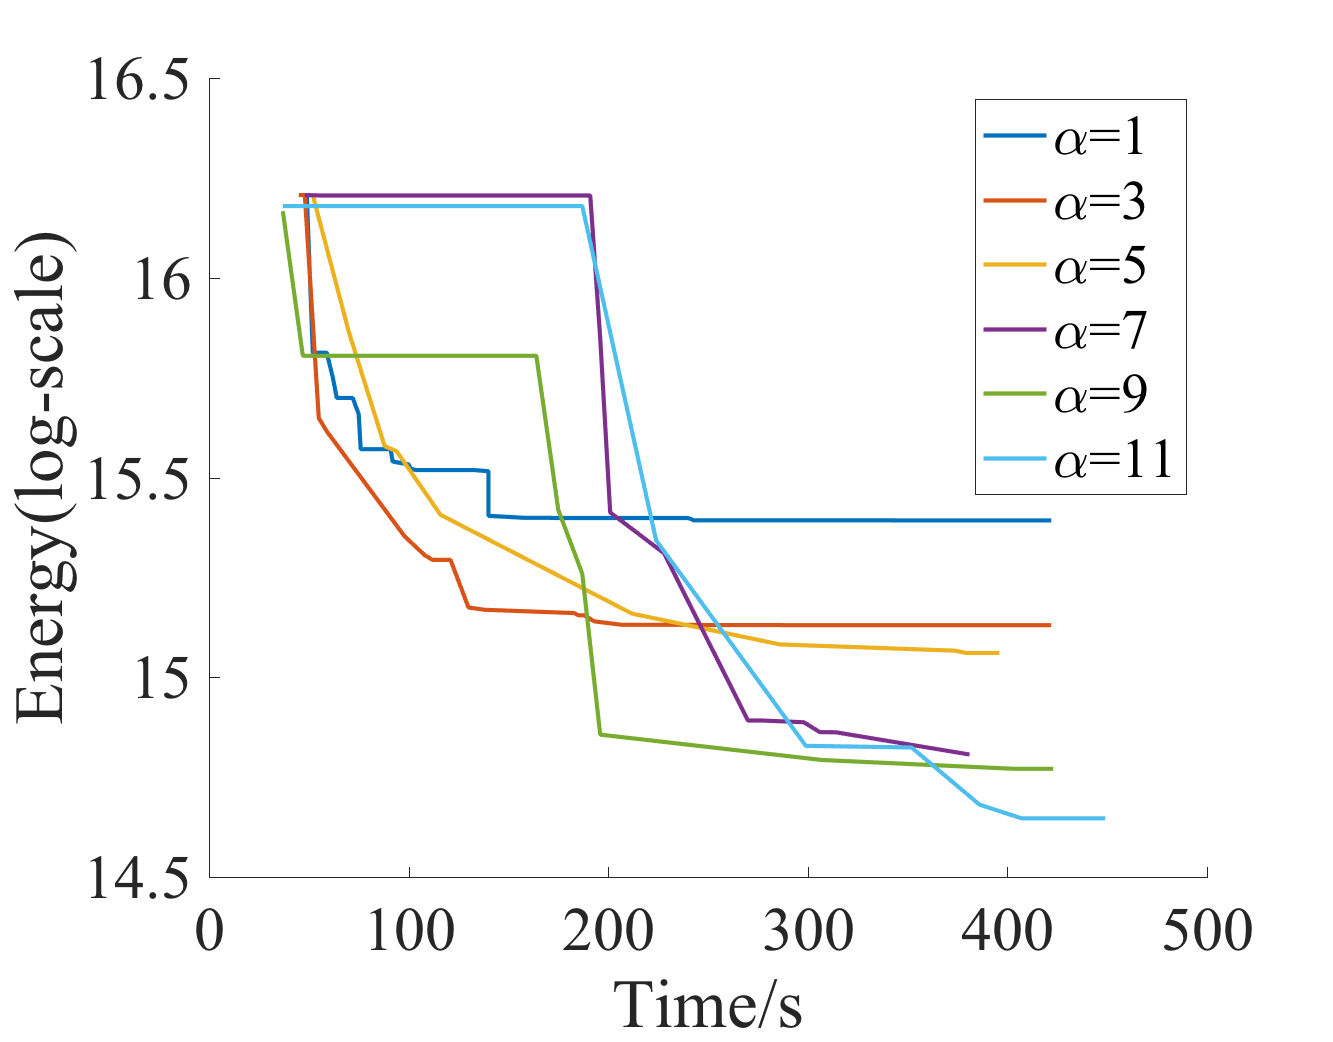
\includegraphics[width=\columnwidth]{figure/layered_depthmap_by_alpha.png}
  \caption{}\label{fig:layered_depthmap_by_alpha}
\end{figure}
\begin{figure}[tb]
  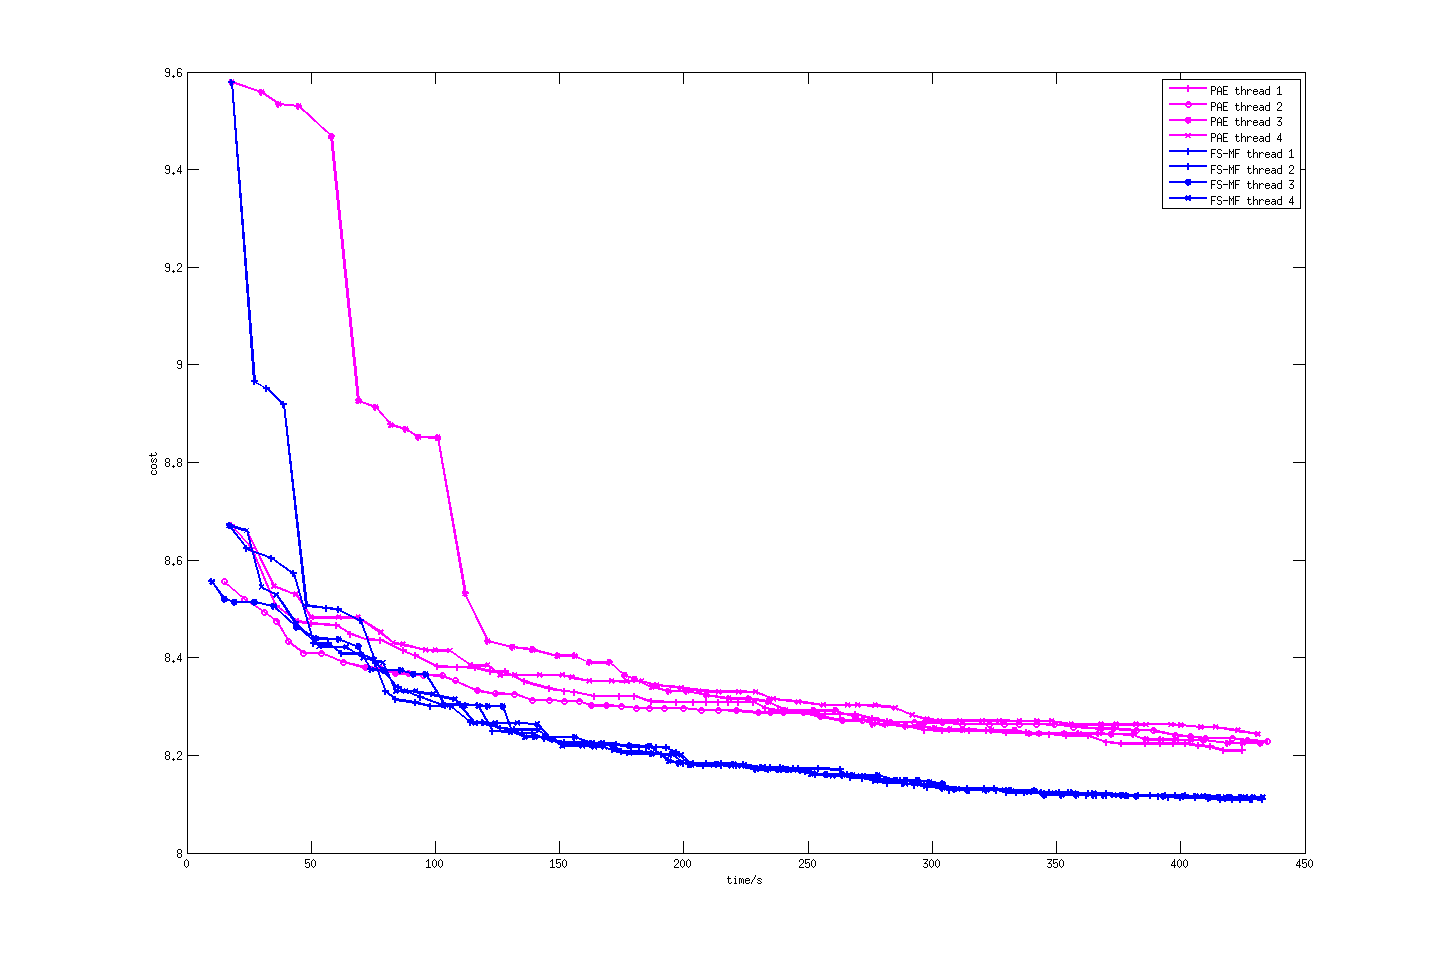
\includegraphics[width=\columnwidth]{figure/optical_flow_by_threads.png}
  \caption{}\label{fig:optical_flow_by_threads}
\end{figure}
\begin{figure}[tb]
  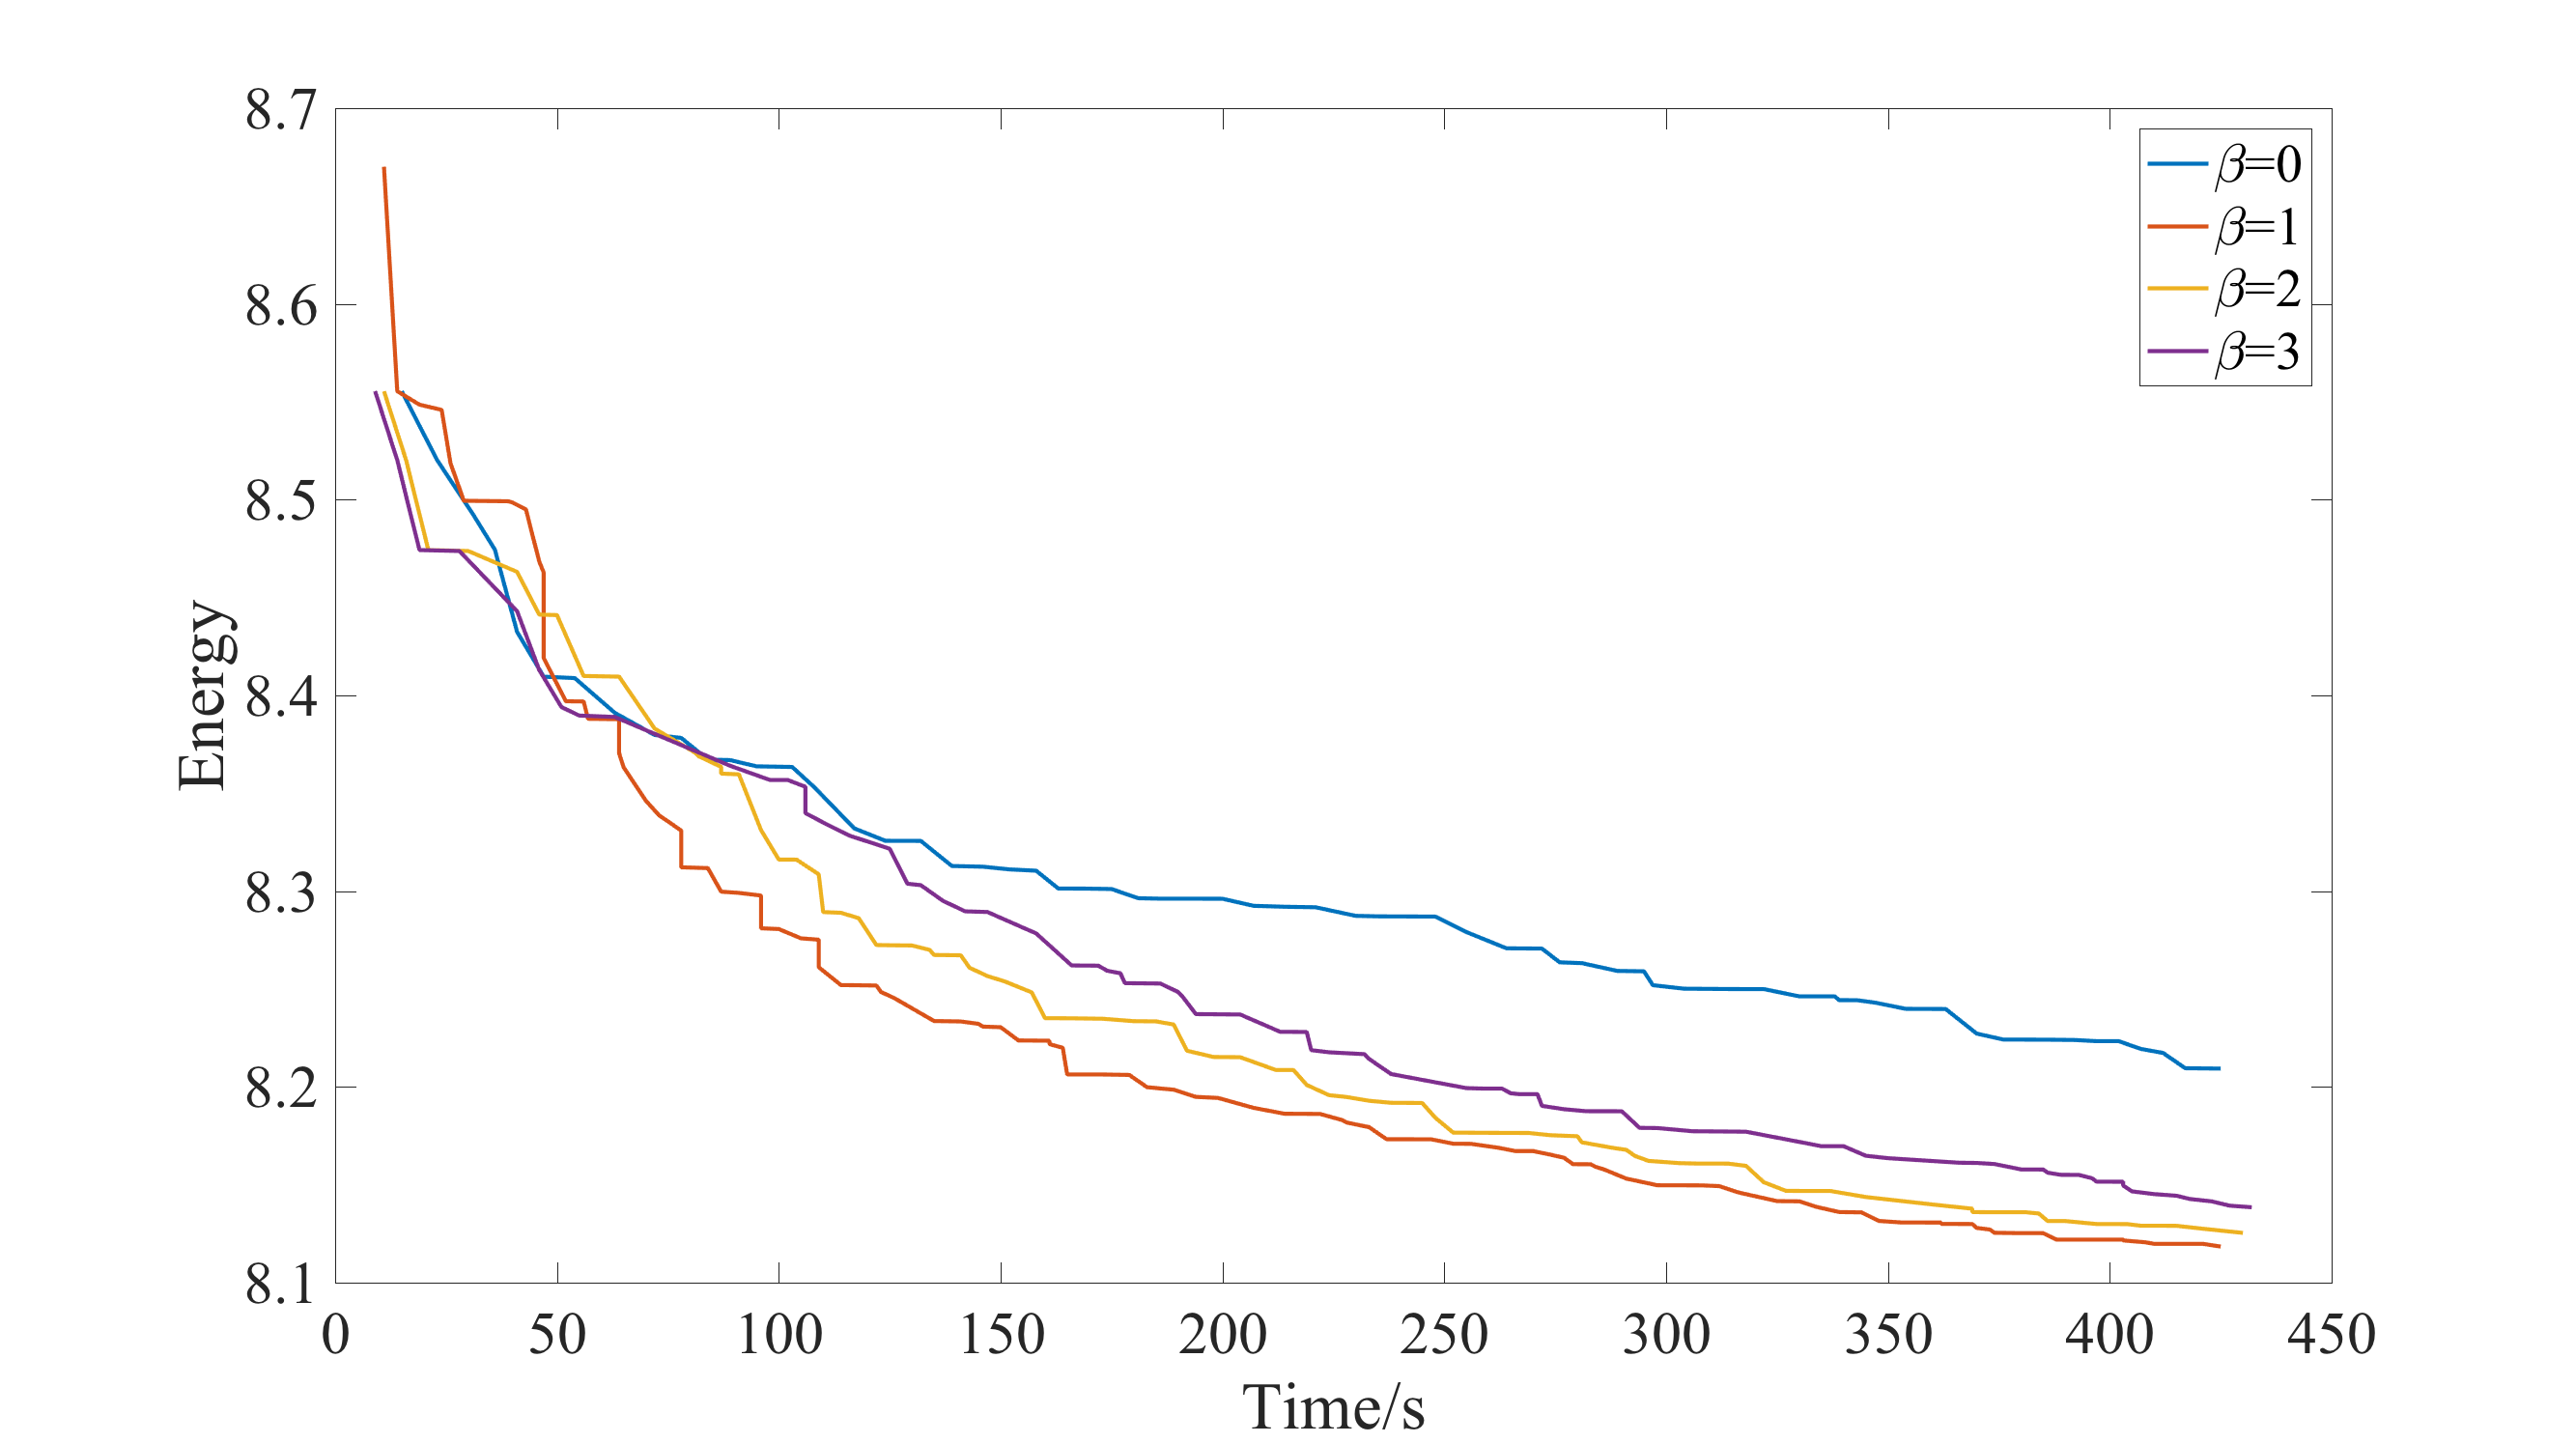
\includegraphics[width=\columnwidth]{figure/optical_flow_by_beta.png}
  \caption{}\label{fig:optical_flow_by_beta}
\end{figure}


\chen{
  There are interesting pattern in the convergence plot of optical flow estimation problem. As both FS-MF and PAE are doing binary fusion, FS-MF finds lower energy faster than PAE. The reason is as follows. Some solution proposals are more effective than others, so once a thread grabs an effective solution proposal, it find a much lower energy. Since there is no solution sharing in PAE model, other threads cannot share this lower energy state, and keeps working on improving its own state. On the other hand, FS-MF allows solution sharing, so once a thread grabs an effective solution proposal and moves to a lower energy state, other threads can share this lower energy state. To further demonstrate what is happening here, we plot the energy-time for each thread in PAE and FS-MF in figure \ref{fig:optical_flow_by_threads}. As we can see from the plots, in PAE model, one thread finds lower energy state faster than others, while other threads keep working at their own energy state. But in FS-MF model, all threads exchange information about the lowest energy state and work on improving the lowest energy state together. So there are more chance of finding effective proposals faster and thus the energy goes down faster. Since the solution for optical flow can be locally improved by each thread, the final merging of PAE can effectively fuse good local results in different threads together and achieve a similar energy state with FS-MF model. Because FS-MF model shares information in the middle, a final merging becomes less necessary. Same comparison holds for FS-SS and FS.
}

\chen{
  To further understand the effect of solution sharing, we did two other experiments. In one experiment, we change the number of solutions each thread grabed from others from 0 to 3 (as there are 4 threads in total) while keeping others the same. The energy-time plot is shown in figure \ref{fig:optical_flow_by_beta}. In another experiment, we change the number of iterations between two consecutive solution sharing iterations as in figure \ref{fig:optical_flow_by_interval}.
}

\chen{
  From the convergence plot of layered depth map estimation, we can see that, Fusion Move, Parallel Fusion Move, and FS-MF all stalk at a high energy state. The reason is binary fusion of solution proposals (either from others or self) is too limited to further decrease the energy due to the complexity of the problem itself. Only when multi-way fusion is used (in FS-SS and FS), it becomes possible for the energy to further decrease. This coincides with the observation in \cite{layered_depthmap} that binary fusion of proposal solutions is not as powerful as their subspace fusion which is a special form of multi-way fusion here. To further explore the effect of multi-way fusion, we use different $\alpha$ {1, 3, 7, 15} in FS model while keeping other parameters the same and plot the energy-time curve in figure \ref{fig:layered_depth_map_by_alpha}.
}

\chen{
  As shown in \ref{section:results}, the multi-way fusion and solution sharing enabled by our uniform framework play a key role for improving performance in different settings. For better understanding our framework, we examine the role played by each factor more closely by varying each factor while keeping others the same. There are four parameters in our framework: \textit{the number of threads}, \textit{the number alpha}, \textit{the number beta}, \textit{the number of iterations between each solution sharing}.
}

